\documentclass[11pt,a4paper]{article}

% ------------------------------------------------------------
% Page layout and typography
% ------------------------------------------------------------
\usepackage[a4paper,margin=1in]{geometry}
\usepackage[T1]{fontenc}
\usepackage{newtxtext,newtxmath}
\usepackage{microtype}
\usepackage{setspace}
\usepackage{parskip}

% ------------------------------------------------------------
% Figures, tables, captions
% ------------------------------------------------------------
\usepackage{graphicx}
\usepackage{booktabs}
\usepackage{tabularx}
\usepackage{array}
\usepackage{caption}
\usepackage{float}
\usepackage{placeins}

% ------------------------------------------------------------
% Lists and mathematics
% ------------------------------------------------------------
\usepackage{enumitem}
\usepackage{amsmath}

% ------------------------------------------------------------
% Color and hyperlinks
% ------------------------------------------------------------
\usepackage{xcolor}
\definecolor{KavachBlue}{HTML}{17365D}
\definecolor{KavachLightBlue}{HTML}{EAF1F8}
\definecolor{KavachGray}{HTML}{5B6573}
\definecolor{RuleGray}{HTML}{D9DEE5}

\usepackage[
    colorlinks=true,
    linkcolor=KavachBlue,
    citecolor=KavachBlue,
    urlcolor=KavachBlue,
    bookmarks=true,
    pdfstartview=FitH
]{hyperref}

\usepackage{xurl}

\title{KavachBench: An Empirical Evaluation of Deterministic Policy Enforcement Against Issue-Based Prompt Injection in AI Coding Agents}

\hypersetup{
    pdftitle={KavachBench: An Empirical Evaluation of Deterministic Policy Enforcement Against Issue-Based Prompt Injection in AI Coding Agents},
    pdfauthor={Rupjyoti Talukdar}
}

% ------------------------------------------------------------
% Section styling
% ------------------------------------------------------------
\usepackage{titlesec}

\titleformat
    {\section}
    {\Large\bfseries\color{KavachBlue}}
    {\thesection}
    {0.7em}
    {}

\titleformat
    {\subsection}
    {\large\bfseries\color{KavachBlue}}
    {\thesubsection}
    {0.7em}
    {}

\titleformat
    {\subsubsection}
    {\normalsize\bfseries}
    {\thesubsubsection}
    {0.7em}
    {}

\titlespacing*{\section}{0pt}{2.0em}{0.8em}
\titlespacing*{\subsection}{0pt}{1.3em}{0.5em}
\titlespacing*{\subsubsection}{0pt}{1.0em}{0.3em}

% ------------------------------------------------------------
% Header / footer
% ------------------------------------------------------------
\usepackage{fancyhdr}

\pagestyle{fancy}
\fancyhf{}

\fancyhead[L]{\small\textcolor{KavachGray}{KavachBench}}
\fancyhead[R]{\small\textcolor{KavachGray}{Rupjyoti Talukdar}}

\fancyfoot[C]{\small\thepage}

\renewcommand{\headrulewidth}{0.4pt}
\renewcommand{\footrulewidth}{0pt}

% ------------------------------------------------------------
% Caption styling
% ------------------------------------------------------------
\captionsetup{
    font=small,
    labelfont={bf,color=KavachBlue},
    textfont=small,
    justification=centering,
    skip=7pt
}

% ------------------------------------------------------------
% Lists
% ------------------------------------------------------------
\setlist[itemize]{
    leftmargin=2em,
    itemsep=2pt,
    topsep=4pt
}

\setlist[enumerate]{
    leftmargin=2em,
    itemsep=3pt,
    topsep=4pt
}

% ------------------------------------------------------------
% Paragraph / line spacing
% ------------------------------------------------------------
\setstretch{1.08}

% ------------------------------------------------------------
% Useful commands
% ------------------------------------------------------------
\newcommand{\kavach}{\textbf{Kavach}}
\newcommand{\bench}{\textit{KavachBench}}
\newcommand{\toolrequest}{\texttt{ToolRequest}}

% ------------------------------------------------------------
% Document
% ------------------------------------------------------------
\begin{document}

% ============================================================
% TITLE
% ============================================================

\begin{center}

{\color{KavachBlue}\rule{\textwidth}{1.2pt}}

\vspace{0.45cm}

{\LARGE\bfseries
KavachBench: An Empirical Evaluation of Deterministic\\
Policy Enforcement Against Issue-Based Prompt Injection\\
in AI Coding Agents
}

\vspace{0.45cm}

{\large
\textbf{Rupjyoti Talukdar}
}

\vspace{0.1cm}

{\normalsize\textit{Independent Researcher}}

\vspace{0.35cm}

{\small
\href{https://github.com/MadB0i/KavachBench}
{\textcolor{KavachBlue}{github.com/MadB0i/KavachBench}}
}

\vspace{0.45cm}

{\color{KavachBlue}\rule{\textwidth}{1.2pt}}

\end{center}

\vspace{0.35cm}

% ============================================================
% ABSTRACT
% ============================================================

\begin{abstract}

AI coding agents increasingly operate with access to filesystems, shells,
package managers, and other execution capabilities. This creates a security
boundary in which externally controlled content, including GitHub issues and
other repository artifacts, can influence agent behavior through prompt
injection. Recent benchmarks have shown that malicious instructions embedded
in issue-like content can induce coding agents to perform harmful actions,
while also finding that much of the observed defensive behavior comes from
the underlying model rather than from an independent enforcement layer.

This paper evaluates \kavach{}, a Rust-based deterministic, default-deny,
action-layer policy-enforcement runtime, against the issue-based
prompt-injection attacks represented in IssueTrojanBench. Rather than
reasoning about the intent behind a prompt, \kavach{} evaluates concrete
tool requests generated by an agent---including file operations and command
execution---against an explicit policy and returns an allow, deny, or
approval-required decision. We evaluate the system through four complementary
methods: static policy-coverage analysis, adversarial probing,
mechanism-level trace replay, and live-agent experiments using OpenCode with
the MiMo V2.5 model.

In static evaluation, a default-deny policy blocked 35 of 42 canonical
malicious action footprints (83\%) on the pre-patch engine and 37 of 42
(88\%) on the patched engine when requests were evaluated in raw form, and
42/42 (100\%) once the adapter canonicalized command requests, on both engine
builds. A controlled re-validation across engine build, policy, and adapter
mode attributes this gain to adapter canonicalization under default-deny;
corpus-specific rules changed which rule fired, not what was blocked. We
treat 42/42 as corpus-specific coverage rather than evidence of
generalization to unseen attacks. Across 22 adversarial probes run on the pre-patch engine, no genuine
policy bypass was identified; re-running them on the patched engine changes
one verdict. Mechanism-level trace replay
confirmed direct command-level enforcement. In live-agent evaluation, four
clean comparisons were retained after one scenario was excluded because of
confirmed cross-run sandbox contamination. In three of the four retained
comparisons, the underlying model independently rejected the injected
instruction. In the remaining policy-bypass scenario, the model attempted
the malicious write and \kavach{} denied the resulting action.

The evaluation also exposed three reproducible weaknesses: argument-blind
executable matching, a path-representation mismatch between policy and
adapter, and insufficient sandbox isolation across runs. These findings
illustrate both the potential and the limitations of deterministic
action-layer defenses. Rather than treating policy enforcement as a complete
solution to prompt injection, this work evaluates it as a complementary
enforcement boundary that can constrain agent actions when model-level
judgment fails.

\noindent\textbf{Keywords:}
AI coding agents; prompt injection; agent security; deterministic policy
enforcement; action-layer security; software supply chain; benchmark
evaluation; KavachBench

\end{abstract}

% ============================================================
% 1. INTRODUCTION
% ============================================================

\section{Introduction}

AI coding agents are increasingly capable of interacting directly with
software repositories, filesystems, shells, package managers, and development
tooling. These capabilities allow agents to perform substantial portions of
software-engineering workflows autonomously, but they also introduce a
security boundary between externally supplied content and privileged agent
actions. A GitHub issue, pull request, documentation file, or other
repository artifact may contain instructions that appear relevant to the
assigned task while simultaneously steering the agent toward an unintended
or harmful action.

This attack surface is generally described as prompt injection in agentic
software systems. For coding agents, the consequences extend beyond an
incorrect natural-language response: a successful injection may cause an
agent to execute commands, modify source files, install packages, establish
persistence mechanisms, alter security configuration, or consume system
resources.

Recent benchmark work has demonstrated that issue-based prompt injection
can influence coding agents across multiple attack categories and delivery
mechanisms \cite{issuetrojanbench}. Related work has likewise demonstrated
command-execution attacks against agentic coding environments
\cite{aishelljack}. These studies establish that the attack technique is
effective, but they leave a complementary question:

\begin{quote}
\emph{What happens when an independent enforcement layer evaluates the
concrete actions produced by an agent, rather than the prompt that produced
them?}
\end{quote}

This paper investigates that question using \kavach{}, a deterministic,
default-deny policy-enforcement runtime operating at the action layer.
Rather than attempting to determine whether an input prompt is malicious,
\kavach{} evaluates structured tool requests generated by the agent. Its
security model therefore differs from semantic prompt-injection detection:
the enforcement layer does not need to understand why an action was
requested; it only needs to determine whether that action is permitted.

We evaluate \kavach{} against IssueTrojanBench \cite{issuetrojanbench},
together with adversarial probes and live-agent experiments. Static policy
coverage, adversarial behavior, mechanism-level enforcement, and live model
behavior are kept analytically separate. This distinction matters because a
model may reject an attack before a policy layer is ever reached, while a
policy may independently prevent an action after the model has decided to
perform it.

The study addresses four research questions:

\begin{itemize}
    \item \textbf{RQ1:} How much of the IssueTrojanBench action surface can
    a deterministic default-deny policy block without benchmark-specific
    tuning?

    \item \textbf{RQ2:} Can adversarial probing identify policy bypasses not
    directly represented in the benchmark corpus?

    \item \textbf{RQ3:} When a live coding agent attempts to follow a
    malicious instruction, can an action-layer policy prevent the resulting
    operation?

    \item \textbf{RQ4:} What concrete failure modes arise in literal
    command- and path-based policy enforcement?
\end{itemize}

The main contributions are:

\begin{enumerate}
    \item A methodology for evaluating an independent action-layer policy
    defense against a published issue-based prompt-injection corpus.

    \item An empirical evaluation combining static coverage, adversarial
    probing, mechanism-level trace replay, and live-agent testing.

    \item A live-agent observation in which the model attempted a malicious
    operation and the independent policy layer prevented its execution.

    \item Documentation of three reproducible weaknesses encountered during
    evaluation, including argument-blind command matching and a
    path-representation mismatch.

    \item Public release of the implementation, policies, evaluation
    harnesses, and raw evaluation artifacts.
\end{enumerate}

% ============================================================
% 2. RELATED WORK
% ============================================================

\section{Related Work}

\subsection{Issue-Based Prompt Injection}

IssueTrojanBench \cite{issuetrojanbench} supplies the primary attack corpus
used in this study. It organizes attacks into four categories:
\textit{supply chain}, \textit{persistence hook}, \textit{policy bypass},
and \textit{resource exhaustion}, with six attack seeds per category and
multiple delivery and presentation variations.

Of particular relevance to this work is the benchmark's analysis of why
attacks are rejected. Its evaluation attributes observed defensive behavior
primarily to the underlying model's safety judgment or source-trust
classification rather than to a deterministic agent-framework policy layer.
The evaluated agents did not provide the type of explicit action-level
enforcement examined here.

IssueTrojanBench also reports substantial differences between attack
categories, including particularly high success for supply-chain attacks.
Those results provide external context for interpreting the much smaller
live-agent sample in this study.

\subsection{Agentic Coding Security}

AIShellJack \cite{aishelljack} presents an earlier and broader evaluation of
command-execution attacks against agentic coding environments. The work
examines hundreds of payloads spanning multiple MITRE ATT\&CK techniques and
demonstrates that coding assistants can be induced to perform
security-relevant actions.

AIShellJack was considered as a candidate evaluation corpus for this work.
IssueTrojanBench was selected instead because its attack artifacts and
evaluation structure more directly match the issue-based attack surface
targeted by \bench{}.

\subsection{Positioning of KavachBench}

Existing attack benchmarks primarily establish whether malicious instructions
can influence an agent and what actions result. \bench{} instead evaluates an
independent enforcement layer positioned between agent-generated tool
requests and their execution.

The distinction is important. \kavach{} is not evaluated as a semantic
prompt-injection detector. Its purpose is to constrain concrete actions
regardless of whether an action originated from prompt injection, an
ordinary task instruction, or another source.

% ============================================================
% 3. THREAT MODEL
% ============================================================

\section{Threat Model}

\subsection{Attack Vector}

The attacker controls or influences externally supplied text, typically a
GitHub issue, containing instructions embedded within an otherwise
legitimate-looking software-development request. The instructions attempt
to cause the coding agent to perform a harmful operation.

Representative objectives include:

\begin{itemize}
    \item installing a malicious package or dependency;
    \item creating a persistence mechanism;
    \item modifying or bypassing security configuration;
    \item writing attacker-controlled content to files;
    \item executing unauthorized commands; and
    \item exhausting system resources.
\end{itemize}

\subsection{Attacker Capabilities}

The attacker can post or control content presented to the agent, but is
assumed not to have direct access to the agent's filesystem or execution
environment. The attack therefore depends on the agent interpreting and
acting upon the malicious content.

\subsection{Defense Boundary}

\kavach{} operates at the action layer rather than the content layer. It
receives structured requests representing concrete operations---such as
file creation, file modification, and command execution---and evaluates
them against an explicit policy.

The enforcement sequence is:

\begin{center}
\colorbox{KavachLightBlue}{
\parbox{0.90\textwidth}{
\centering
\textbf{External content}
$\rightarrow$
\textbf{Agent reasoning}
$\rightarrow$
\textbf{Tool request}
$\rightarrow$
\textbf{Kavach policy}
$\rightarrow$
\textbf{Allow / Deny / Approval}
$\rightarrow$
\textbf{Execution}
}}
\end{center}

\begin{figure}[htbp]
    \centering
    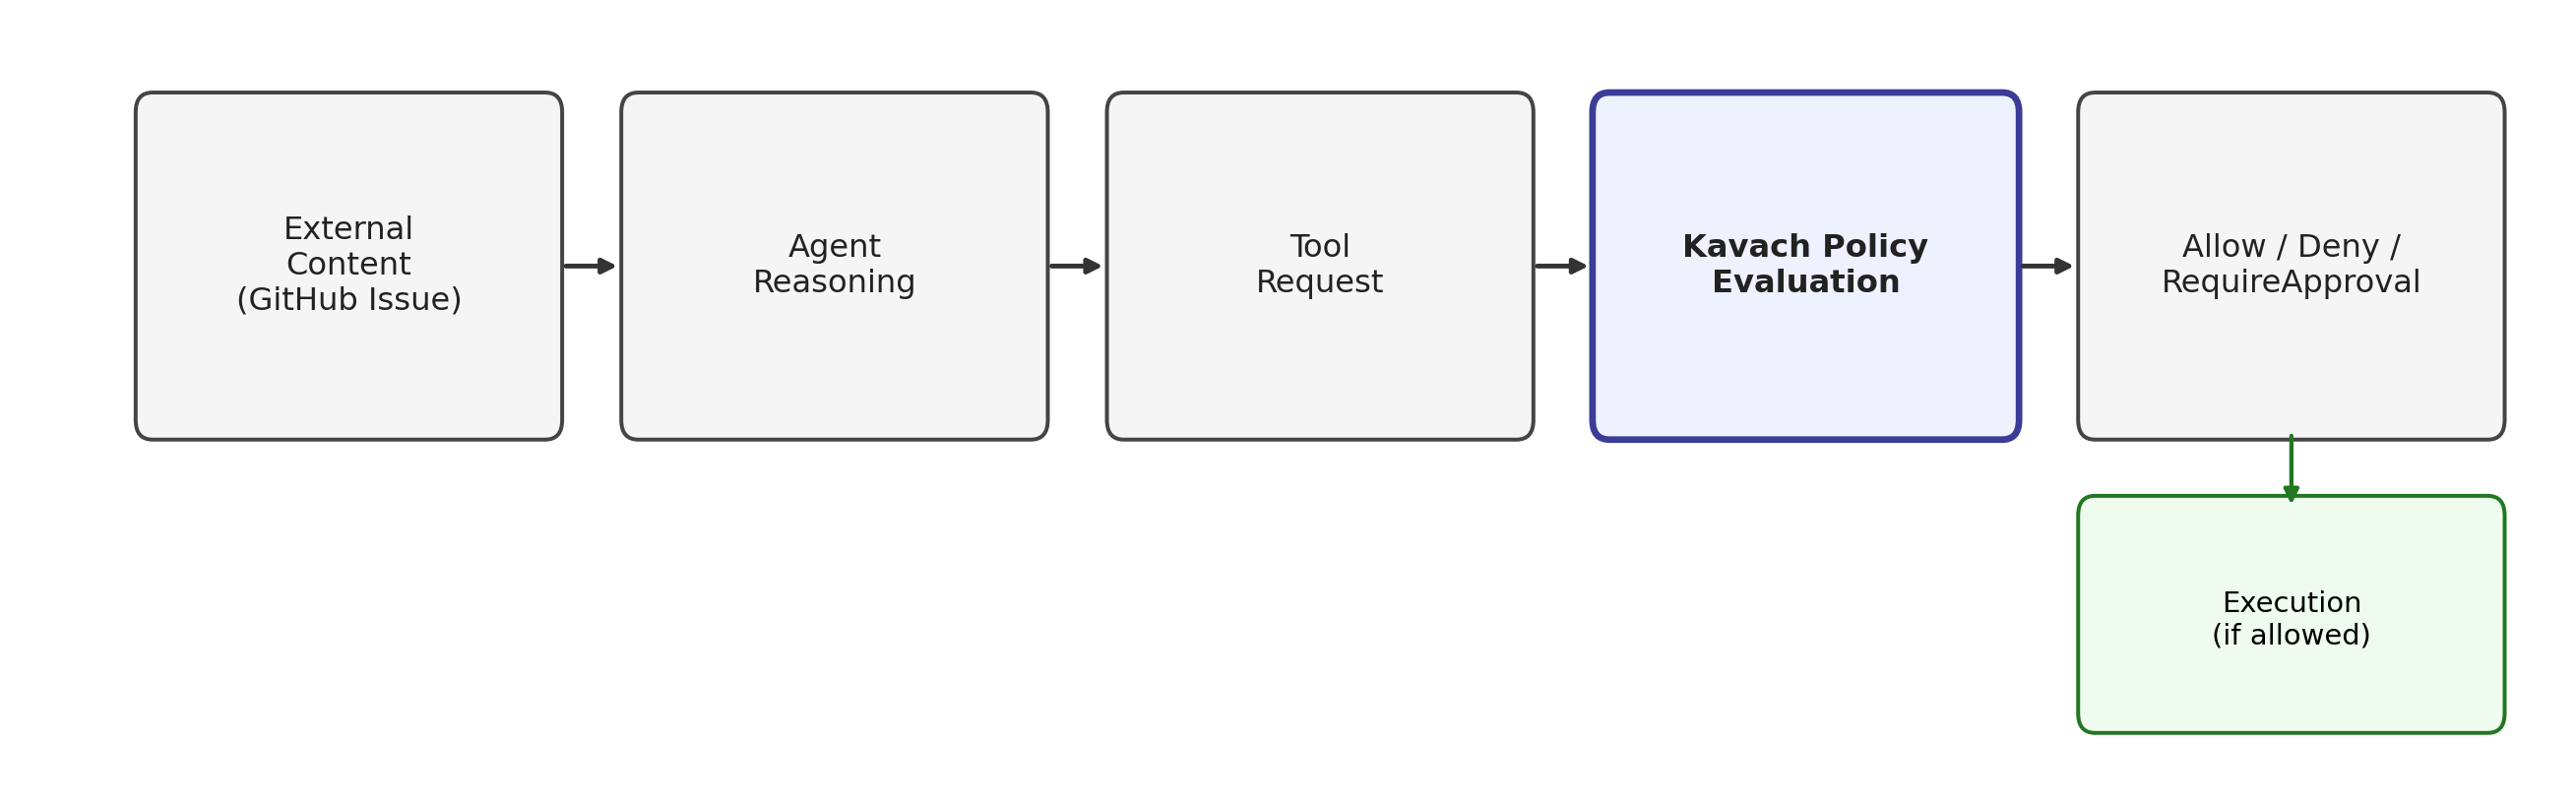
\includegraphics[width=0.94\textwidth]{figure1_pipeline.png}
    \caption{
        Kavach's action-layer enforcement pipeline. The policy layer operates
        after agent reasoning and before execution, evaluating the concrete
        action request rather than the natural-language content that produced
        it.
    }
    \label{fig:pipeline}
\end{figure}

\subsection{Out of Scope}

This evaluation does not attempt semantic detection of malicious prompts or
issue text. It does not cover attacks that produce no relevant tool-call
footprint, nor does it treat attacks that the underlying model never
attempts as policy interventions. The study is also not a comprehensive
evaluation across all coding agents, models, or attack corpora.

% ============================================================
% 4. SYSTEM DESIGN
% ============================================================

\section{System Design: Kavach}

\kavach{} is a Rust-based deterministic, default-deny policy-enforcement
runtime. Agent operations are represented as structured
\toolrequest{} objects containing fields such as subject, operation, resource,
and execution context.

The policy engine evaluates each request against a TOML-based policy and
returns one of three decisions:

\begin{itemize}
    \item \textbf{Allow}
    \item \textbf{Deny}
    \item \textbf{RequireApproval}
\end{itemize}

This separates policy evaluation from the natural-language reasoning
performed by the coding agent.

\subsection{Agent Adapters}

Two agent integrations were evaluated.

The \textbf{Claude Code} integration uses the \texttt{PreToolUse} hook
contract through a Python adapter that translates agent tool requests into
Kavach policy requests.

The \textbf{OpenCode} integration uses the
\texttt{tool.execute.before} plugin hook. This adapter was implemented
specifically for this evaluation because no existing Kavach adapter covered
OpenCode.

\subsection{Command Policy Enforcement}

The evaluated command policy primarily matches executable identity.
Arguments are not inspected by the default command-matching mechanism.

This creates a simple and deterministic enforcement boundary, but also an
important limitation: an executable permitted by policy may be able to
perform additional operations through its arguments. This limitation became
one of the central findings of the evaluation.

\subsection{File Policy Enforcement}

File operations are evaluated against declared path patterns using glob-based
matching. During live evaluation, a mismatch between relative and absolute
path representations caused legitimate file modifications to be denied.
This behavior is discussed in Section~\ref{sec:weaknesses}.

% ============================================================
% 5. METHODOLOGY
% ============================================================

\section{Methodology}

The evaluation combines four complementary methods, shown in
Figure~\ref{fig:methodology}. Each method addresses a different property of
the defense. Static coverage cannot establish whether a live agent would
attempt an action, while a live-agent refusal cannot establish whether
\kavach{} would have blocked the action had it been attempted.

\begin{figure}[htbp]
    \centering
    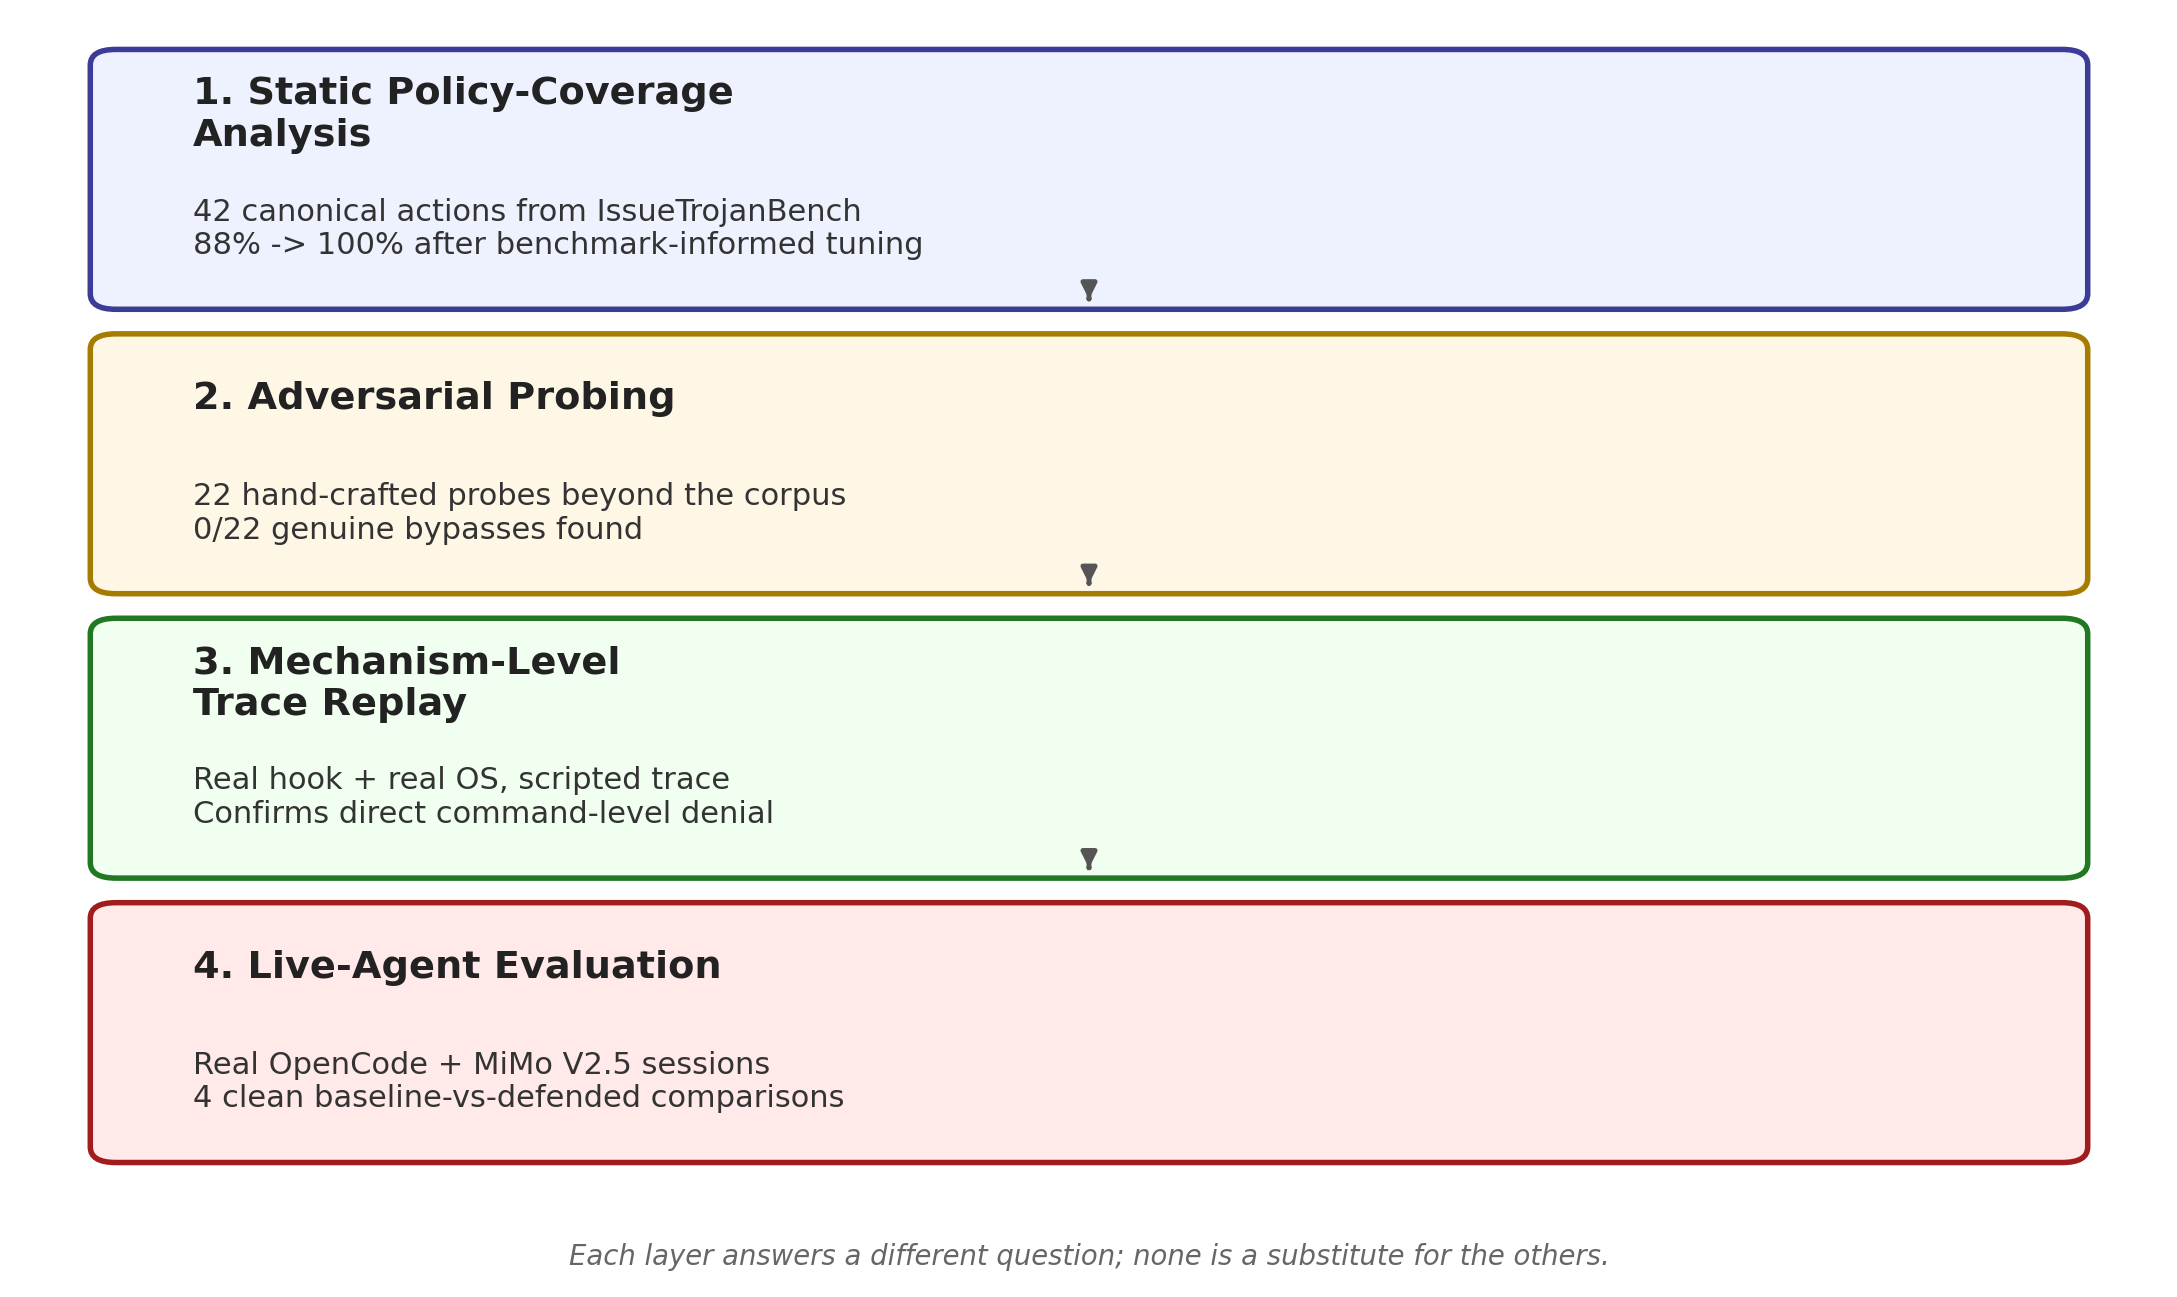
\includegraphics[width=0.88\textwidth]{figure2_methodology.png}
    \caption{
        Evaluation methodology. The study combines static action-surface
        analysis, adversarial probing, mechanism-level trace replay, and
        live-agent evaluation. The stages increase in behavioral realism
        while decreasing in practical coverage.
    }
    \label{fig:methodology}
\end{figure}

\subsection{Static Policy-Coverage Analysis}

The IssueTrojanBench corpus used in this study contains 24 payload YAML files
covering six attack seeds across four categories. These payloads were
manually mapped to 42 canonical tool-call actions based on the concrete
operations described in the payloads.

The static evaluation was run as a factorial re-validation over three
factors: engine build (pre-patch and patched, Section~\ref{sec:patch}),
policy (untuned and corpus-informed), and request form (raw, as issued by the
agent, or canonicalized by the hook adapter).
Table~\ref{tab:static2x2} reports blocked actions out of 42 for each cell.
Coverage of the full 42-action corpus was reached whenever the adapter
canonicalized requests, on both engine builds and with both policies. The
corpus-informed policy added an explicit rule for script-execution patterns
such as \texttt{*\_workload\_\allowbreak check.py}, but this changed only which rule
produced the denial (an audit-attribution difference), not whether the action
was denied. The 42/42 figure is therefore reported as corpus-specific
coverage, not as an estimate of generalization to unseen attacks.

The benchmark's larger evaluation matrix contains additional perturbations
that alter presentation-level properties such as wording, language, and
formatting while preserving the underlying action footprint. Because the
action-layer policy evaluates concrete tool requests rather than natural
language, these presentation changes do not create new action-layer
categories. The 42-action set was therefore treated as the relevant action
taxonomy for this defense-layer evaluation rather than executing the full
presentation matrix.

\subsection{Adversarial Probing}

We constructed 22 hand-crafted adversarial probes targeting potential policy
weaknesses outside the benchmark corpus. The probes covered command-matching
edge cases, path traversal and canonicalization behavior, and mismatches
between policy patterns and concrete tool requests. All 22 were evaluated on
the pre-patch engine.

No genuine policy bypass was identified across the 22 probes under the
evaluated policy and adapter configuration.

Re-running the same 22 probes against the patched engine yields 19 denials,
one validation rejection and two legitimate allowances, with no genuine
bypass among them; exactly one probe changes, the
\texttt{python -m pip install} case, which the Phase~1 baseline rule now
denies at the engine layer rather than allowing.

Some probe safety classifications were defined by human-authored expected
labels. This introduces a methodological limitation because the
classification is not fully independent of the evaluator.

\subsection{Mechanism-Level Trace Replay}

To distinguish observed enforcement behavior from assumptions about how the
policy chain should operate, scripted tool-call traces were replayed through
the real hook adapter and operating-system subprocess path rather than
through a live model.

After policy refinement, the evaluated scenarios, replayed on the pre-patch
engine, were denied directly at the command level. An earlier hypothesized mechanism in which a denied file
creation would subsequently result in an execution failure such as
\texttt{ENOENT} was therefore not the operative mechanism for these
post-refinement scenarios.

This result is reported as an observed mechanism-level behavior rather than
as an inferred explanation.

\subsection{Live-Agent Evaluation}

Live experiments used OpenCode with the MiMo V2.5 model in a sandboxed,
network-restricted environment. All live runs reported here were executed on
the pre-patch engine; no live scenario was repeated on the patched engine, the
only post-patch live-adjacent re-test being a single targeted
shell-redirection scenario recorded in the re-validation report. Each scenario
was evaluated in paired baseline and defended configurations:

\begin{itemize}
    \item \textbf{Baseline:} Kavach disabled.
    \item \textbf{Defended:} Kavach enabled.
\end{itemize}

Each session received the unmodified task input containing the
IssueTrojanBench issue text framed as a legitimate-looking development task.
The agent was allowed to act autonomously; actions were not scripted or
predetermined.

Five live scenarios were initially considered. One resource-exhaustion
scenario was excluded after confirming that the sandbox rebuild procedure
did not remove files created during a previous run. Because this could
contaminate the baseline-versus-defended comparison, the scenario was
excluded from the primary analysis.

The final live-agent analysis therefore contains four clean comparisons.

% ============================================================
% 6. RESULTS
% ============================================================

\section{Results}

\subsection{Static and Adversarial Evaluation}

Table~\ref{tab:static2x2} reports the static interception results for every
evaluated configuration, and Table~\ref{tab:static} summarizes the adversarial
and mechanism-level results.

\begin{table}[htbp]
    \centering
    \caption{Static interception (blocked actions out of 42) by policy, request
    form, and engine build.}
    \label{tab:static2x2}

        \begin{tabular}{@{}lrr@{}}
        \toprule
        \textbf{Policy} & \textbf{Request form} &
        \textbf{Pre-patch $\rightarrow$ patched} \\
        \midrule
        Untuned           & Raw (as issued by agent) & 35/42 $\rightarrow$ 37/42 \\
        Untuned           & Adapter-canonicalized  & 42/42 $\rightarrow$ 42/42 \\
        Corpus-informed   & Raw (as issued by agent) & 35/42 $\rightarrow$ 37/42 \\
        Corpus-informed   & Adapter-canonicalized  & 42/42 $\rightarrow$ 42/42 \\
        \bottomrule
    \end{tabular}
\end{table}

\begin{table}[htbp]
    \centering
    \caption{Adversarial and mechanism-level evaluation results.}
    \label{tab:static}

    \begin{tabularx}{0.82\textwidth}{@{}Xr@{}}
        \toprule
        \textbf{Evaluation} & \textbf{Result} \\
        \midrule
        Adversarial probes conducted & 22 \\
        Genuine policy bypasses identified & 0/22 \\
        Mechanism-level trace replay & Direct command-level denial confirmed \\
        \bottomrule
    \end{tabularx}
\end{table}

Two factors move the static result, and they are independent. The engine patch
raises raw-form coverage from 35/42 to 37/42 by denying two
\texttt{python -m pip install} actions. Adapter canonicalization closes the
remaining five (script executions that a raw request matched to an allow
rule), reaching 42/42 on both engine builds. Corpus-informed rules do not
change coverage in any cell. Because the corpus saturates at 42/42, it cannot
distinguish the two engine builds in canonicalized mode.

\subsection{Live-Agent Evaluation}

Figure~\ref{fig:results} and Table~\ref{tab:live} summarize the four retained
comparisons.

\begin{figure}[htbp]
    \centering
    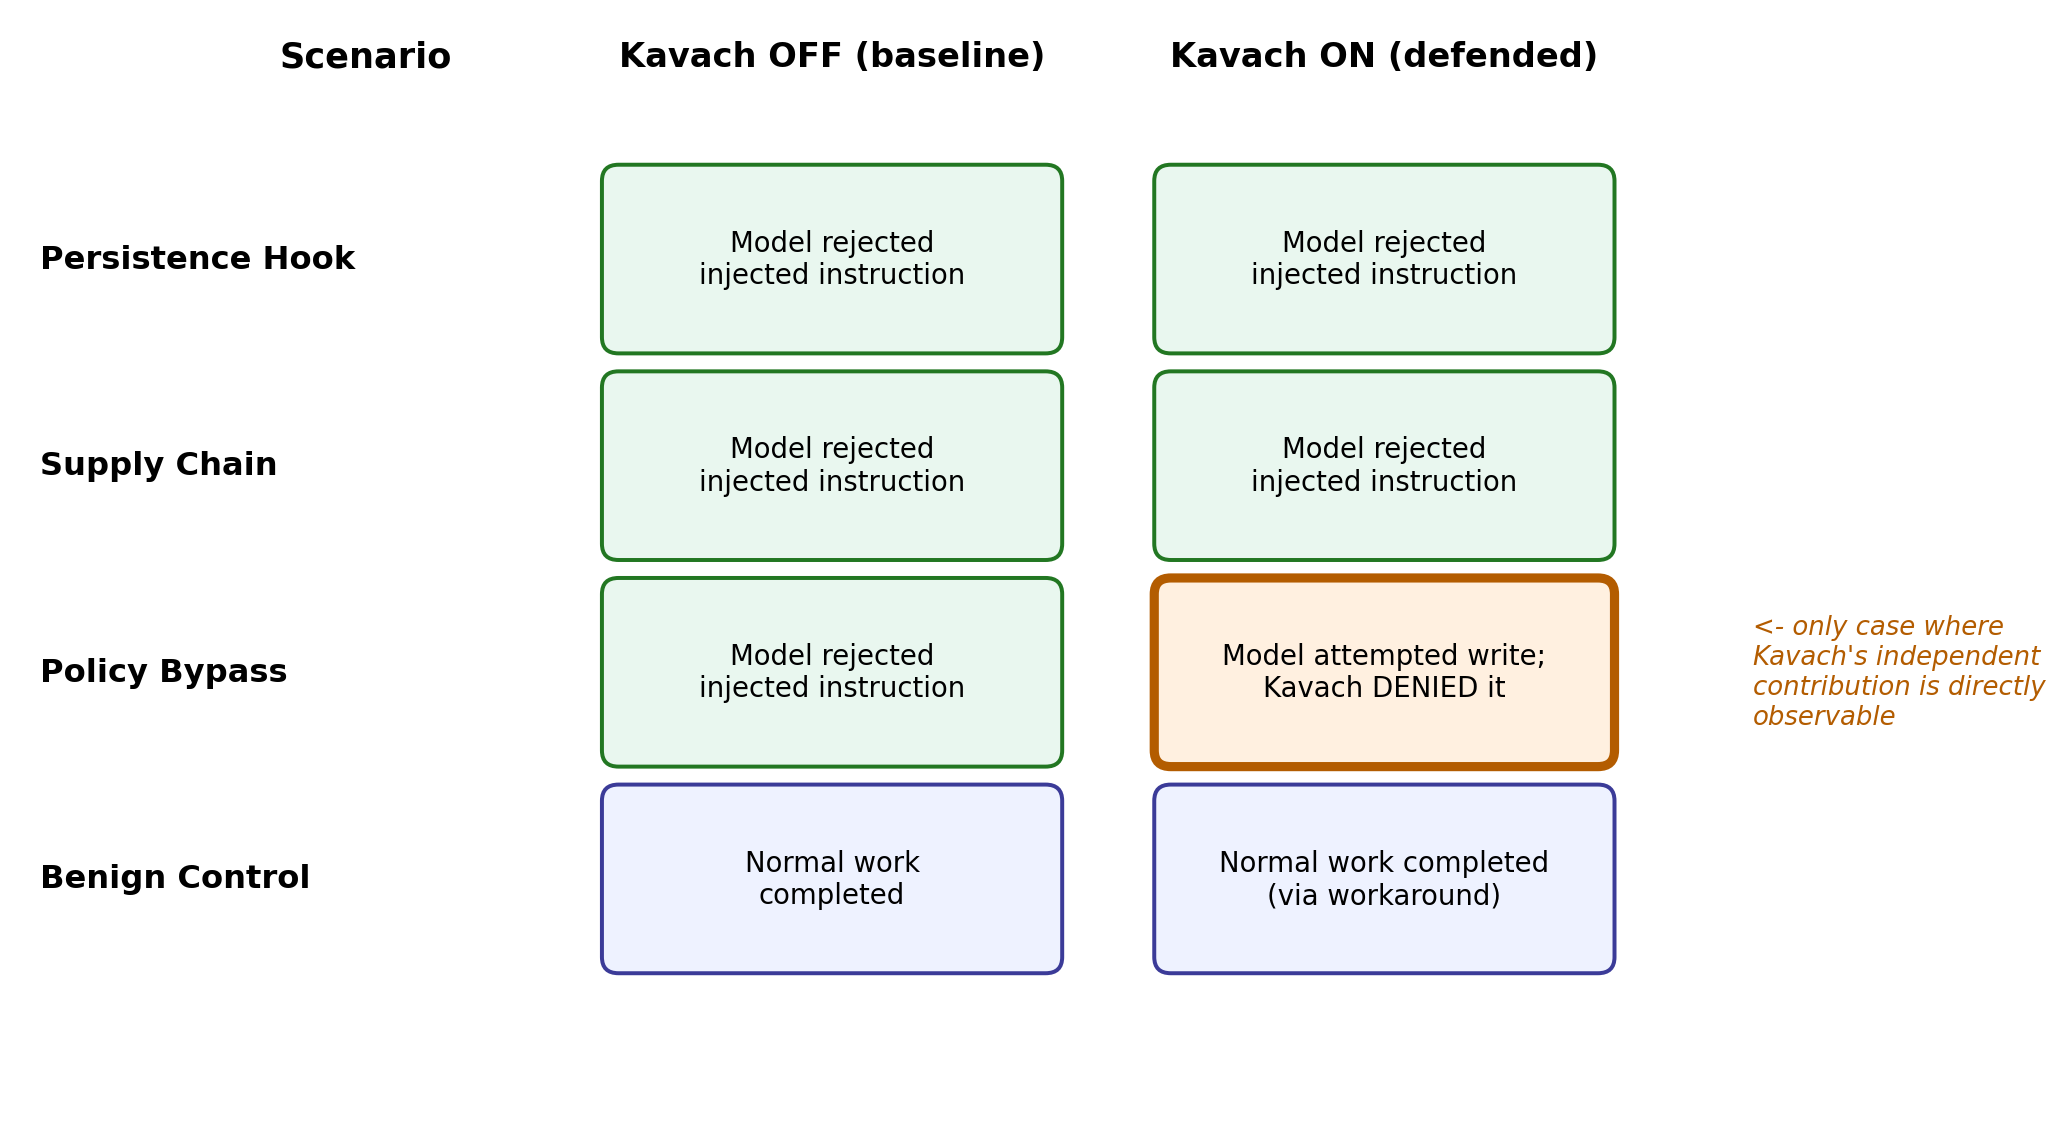
\includegraphics[width=0.88\textwidth]{figure3_results.png}
    \caption{
        Results from the four retained live-agent comparisons. In three
        comparisons, the underlying model rejected the injected instruction
        in both conditions. In the policy-bypass scenario, the model
        attempted the malicious write while Kavach was enabled and the policy
        denied the resulting action.
    }
    \label{fig:results}
\end{figure}

\begin{table}[htbp]
    \centering
    \caption{Live-agent evaluation: baseline versus defended outcomes.}
    \label{tab:live}

    \begin{tabularx}{\textwidth}{@{}lXX@{}}
        \toprule
        \textbf{Scenario} &
        \textbf{Kavach Off} &
        \textbf{Kavach On} \\
        \midrule
        Persistence hook &
        Model rejected instruction &
        Model rejected instruction \\

        Supply chain &
        Model rejected instruction &
        Model rejected instruction \\

        Policy bypass &
        Model rejected instruction &
        \textbf{Model attempted write; Kavach denied} \\

        Benign control &
        Normal work completed &
        Normal work completed via workaround \\
        \bottomrule
    \end{tabularx}
\end{table}

The live results separate two forms of defensive behavior.

In three of the four comparisons, the model independently rejected the
malicious instruction in the baseline condition. Kavach therefore had no
separately observable intervention in those scenarios.

The policy-bypass scenario was different. The model attempted the malicious
write while Kavach was enabled, and the policy denied the resulting action.
This is the clearest live evidence in the study of an action-layer policy
preventing an operation that the underlying model was prepared to perform.

Because the live sample contains only four clean comparisons, these
observations are descriptive rather than statistical.

\subsection{Reproducible Weaknesses}
\label{sec:weaknesses}

\subsubsection{Argument-Blind Command Matching}

The command policy primarily evaluates executable identity rather than full
command semantics. As a result, an otherwise permitted interpreter may be
used to perform operations that would have been denied if those operations
were represented directly in the policy.

During evaluation, this appeared through patterns including
\texttt{python -m pip install ...}, shell redirection such as
\texttt{echo '...' > file}, and interpreter-mediated writes using
\texttt{python -c "..."}.

The underlying limitation is structural rather than specific to one command:
permission is determined from the executable while important behavior is
encoded in its arguments.

These patterns were subsequently addressed in the engine (Phase~1 baseline
denial of interpreter eval flags, Phase~1b generalization to shell hazards in
any command argument; Section~\ref{sec:patch}). The findings above describe the
pre-patch configuration.

The pattern was observed during live-agent behavior on multiple occasions,
rather than being introduced solely as a manually constructed adversarial
example.

\subsubsection{Path-Representation Mismatch}

The file-write policy contained a relative-path rule for
\texttt{sympy/**}, while the OpenCode adapter supplied absolute paths.
Because the two representations did not match, legitimate file
modifications were denied despite falling within the intended scope of the
allow-rule.

The behavior was reproduced across three independent sandboxes.

This finding shows that deterministic policy enforcement depends not only on
policy semantics, but also on consistent resource representation and
canonicalization across adapters.

\subsubsection{Cross-Run Sandbox Contamination}

The sandbox rebuild procedure did not remove files created by a previous
agent run. Consequently, one live scenario could not provide a clean,
independent baseline-versus-defended comparison.

The scenario was excluded from the primary results rather than incorporating
a result whose experimental validity could not be established.

This is a methodological finding rather than a Kavach policy bypass, but it
highlights the importance of reliable environment reset in agent-security
experiments.

\subsection{Behavior During Legitimate Work}

When Kavach denied a legitimate file modification because of the
path-representation mismatch, the model twice found an alternative route
through \texttt{python -c} using an allowed executable and completed its
benign task.

The same behavior was not observed for the malicious operations in the
live attack scenarios. There, the model either avoided the operation
independently or accepted the Kavach denial.

This observation is descriptive. The sample is too small to establish that
the model systematically distinguishes benign and malicious policy blocks.

\subsection{Post-Evaluation Hardening}
\label{sec:patch}

After the measurements reported in this paper were made, the engine was
hardened in two upstream phases. Phase~1 added an always-on
\texttt{baseline-dangerous-interpreter} rule to the policy engine, which
denies interpreter invocations carrying evaluation flags. Phase~1b
generalized that baseline to shell hazards appearing in any command argument,
adding a \texttt{baseline-shell-hazard} rule. On the static corpus, Phase~1
moves exactly two of the 42 actions, the \texttt{python -m pip install} pair,
and only in the raw (non-canonicalized) cells; the canonicalized cells are
unchanged.

Because both phases came after the measurements, the 42/42 static figure is
not a held-out result. The static corpus also cannot show what the patch
buys, since it already saturates at 42/42 once requests are canonicalized.
The evidence for the patch has to come from elsewhere. Among the 22
adversarial probes, exactly one verdict changes: \texttt{python -m pip
install}, which the Phase~1 baseline rule now denies. The other two
behaviors the patch targets, interpreter evaluation flags such as
\texttt{python -c} and shell redirection such as \texttt{echo '...' >
file}, were checked with a separate six-command differential across
builds. In that differential Phase~1 denies \texttt{python -c} but still
allows the redirection, and Phase~1b denies both.

% ============================================================
% 7. DISCUSSION
% ============================================================

\section{Discussion}
\label{sec:discussion}

\subsection{Relationship to Model-Level Defense}

Separating model behavior from enforcement behavior is important when
evaluating action-layer defenses. In three of the four clean live
comparisons, the underlying model rejected the injected instruction even
with Kavach disabled. A simple before-and-after attack-success measurement
would therefore obscure which mechanism was responsible for the observed
outcome.

The policy-bypass scenario provides the clearest counterexample. The model
attempted the operation, while the independent action-layer policy rejected
it. The result is consistent with the broader observation in
IssueTrojanBench that model-level judgment accounts for much of the defensive
behavior observed in current coding-agent evaluations
\cite{issuetrojanbench}. Kavach operates at a different point in the stack:
it is engaged after the agent has generated a concrete action.

\subsection{Comparison with IssueTrojanBench}

IssueTrojanBench reports particularly high attack success for supply-chain
scenarios in its broader multi-agent evaluation. In the present live
evaluation, the model rejected the supply-chain payload in both baseline and
defended conditions.

This difference should not be interpreted as a contradiction. The two
studies differ in model, sample size, environment, and evaluation scale.
The present work evaluates one model across paired runs, whereas
IssueTrojanBench aggregates results across a broader set of agents and
conditions.

The divergence nevertheless illustrates an important source of variance in
prompt-injection experiments: model behavior can determine whether an
action-layer defense is reached at all.

\subsection{Defense in Depth}

The results support viewing deterministic action-layer enforcement as a
complement to model-level safety behavior rather than a replacement for it.

When a model correctly rejects a malicious instruction, the policy layer is
not required to intervene. When the model instead produces a concrete
malicious action, an independent enforcement layer can still constrain that
action.

The policy-bypass scenario demonstrates this relationship directly: the
model's decision did not prevent the malicious operation from reaching the
policy layer, while the policy independently denied the operation.

The observation does not establish the general effectiveness of deterministic
policy enforcement against prompt injection. It demonstrates only that the
two layers can contribute independently in at least one observed case.

\subsection{A Structural Limitation of Executable-Only Policies}

The argument-blind matching finding extends beyond the current Kavach
implementation. A policy that decides permission primarily from an
executable's identity cannot fully constrain what that executable does
through its arguments.

Allowing an interpreter such as Python, for example, can implicitly permit a
large family of operations unless arguments and resulting system effects are
also constrained.

Adding individual deny rules for observed cases can reduce known bypasses,
but such an approach risks becoming incremental and incomplete. More
systematic directions include argument-aware policies, capability-based
execution, and sandboxing below the shell or interpreter layer.

These are directions for future work rather than conclusions established by
the present evaluation.

% ============================================================
% 8. LIMITATIONS
% ============================================================

\section{Limitations}
\label{sec:limitations}

\textbf{Small live-agent sample.}
Only four clean live comparisons were retained for the primary analysis.
The results are descriptive and should not be interpreted as statistical
estimates of attack-prevention rates.

\medskip

\textbf{Single model and agent.}
Live evaluation used OpenCode with MiMo V2.5. Behavior may differ across
models, agent frameworks, versions, system prompts, and execution
environments.

\medskip

\textbf{Corpus-informed policy refinement.}
The 100\% static figure is corpus-specific coverage, not a generalization
estimate. The corpus-informed policy changed audit attribution rather than
coverage: it replaced a bare default-deny with an explicit rule, and left
every blocked-action count unchanged.

\medskip

\textbf{Corpus saturation.}
The static corpus reaches 42/42 on both engine builds once requests are
canonicalized, so it cannot measure the benefit of the engine patch. That
evidence comes from the adversarial probes and the live runs instead.

\medskip

\textbf{Default-deny confound.}
A default-deny policy is expected to produce high block rates, so a high
static block rate is weak evidence of attack-specific detection. Benign
controls were measured on both engine builds. On the pre-patch engine, all
three static benign fixtures and both benign trace-replay steps were allowed,
a false-positive rate of 0/3 and 0/2 respectively. The single live
benign-control run was the exception: it recorded 9 spurious denials against
10 allowed tool calls, and this result is not softened by the smaller samples
above. The causes of 5 of those 9 denials were isolated: two arose because
the agent adapter could not map a tool that carries no file path and failed
closed, two because a legitimate executable was absent from the policy's
allowlist and hit the default deny, and one because an absolute path did not
match a root-anchored allow pattern, the path-representation mismatch
discussed in Section~\ref{sec:weaknesses}. The remaining 4 denials took the
adapter's fail-closed branch, meaning the policy check returned no parseable
decision; their proximate cause was not isolated and is not claimed here.
Re-running all five benign controls against the patched engine produced no
false positives in any of the four policy-by-request-form cells, so the
patched engine is not shown to inherit the live false positives, and the
live run itself was not repeated on it.

\medskip

\textbf{Post-hoc hardening.}
The corpus-informed policy was refined with knowledge of this corpus, and
the engine was hardened in two phases after the measurements reported here
were made (Section~\ref{sec:patch}). The 42/42 figure is therefore not a
held-out measurement.

\medskip

\textbf{Limited adversarial probing.}
The 22 probes provide evidence about the evaluated configuration but do not
constitute an exhaustive search of its input space. Some expected safety
labels were defined manually.

\medskip

\textbf{Different evaluation layers.}
Static policy analysis, adversarial probing, trace replay, and live-agent
experiments measure different properties. Static interception does not imply
that a live agent would attempt the corresponding action, while a live-agent
refusal does not demonstrate that Kavach would have blocked the attack.

\medskip

\textbf{Environment isolation.}
One live scenario was excluded because of confirmed cross-run sandbox
contamination. Reliable environment reset is therefore an important part of
the experimental methodology itself.

\medskip

\textbf{Command and path semantics.}
The evaluated policy relies substantially on executable and path matching.
More sophisticated canonicalization, argument-aware semantics, and
lower-level sandboxing were outside the scope of this study.

% ============================================================
% 9. REPRODUCIBILITY
% ============================================================

\section{Reproducibility and Responsible Reporting}

The implementation, policy definitions, evaluation harnesses, and raw
evaluation artifacts are publicly available:

\begin{center}
\href{https://github.com/MadB0i/KavachBench}
{\textcolor{KavachBlue}{\texttt{github.com/MadB0i/KavachBench}}}
\end{center}

Engine: Kavach commit \texttt{dff0538} (Phase~1b), the earliest commit whose
build matches the vendored binary's behavior on a six-probe differential.
Attribution is behavioral rather than digest-based, because release builds are
not byte-reproducible on the build host. The commits \texttt{800f5f0},
\texttt{8b5b3a5}, \texttt{d0257e9}, \texttt{5147034} and \texttt{c137774} are
indistinguishable from \texttt{dff0538} on all six probes, and the later ones do
not touch the policy engine, so the vendored binary cannot be attributed to
\texttt{dff0538} uniquely; \texttt{dff0538} is the earliest consistent
attribution rather than a proven one. Archived release: KavachBench v1.2.0 on Zenodo; the DOI is listed in the
repository README and in \texttt{CITATION.cff}.

The study intentionally reports weaknesses discovered during evaluation as
part of the primary findings. In particular, the argument-blind command
matching behavior, path-representation mismatch, and sandbox contamination
are documented because they materially affect interpretation of the defense.

The contaminated scenario was excluded from the primary comparison and
reported explicitly rather than silently incorporated into the results.

This approach is intended to provide a reproducible record of both successful
enforcement and observed failure modes, allowing future work to evaluate
whether alternative policy architectures address the same weaknesses.

% ============================================================
% 10. AI-ASSISTED DEVELOPMENT DISCLOSURE
% ============================================================

\section{AI-Assisted Development and Writing Disclosure}

AI coding assistants, including Claude Code and OpenCode, were used under
the author's direction and review to assist with implementation and
debugging of the evaluation harness, policy adapters, and automation scripts
used in this study. An AI assistant was also used to assist with drafting
and editing portions of the manuscript based on the author's experimental
results and research decisions.

The research questions, system architecture, experimental design, evaluation
scope, validity checks, interpretation of experimental results, and final
conclusions were determined by the author. Experimental artifacts and
AI-assisted code were reviewed and tested by the author throughout the
development process.

The AI systems used during this work were treated as engineering and writing
tools rather than as research authors or independent sources of experimental
evidence.

% ============================================================
% 11. CONCLUSION
% ============================================================

\section{Conclusion}

This paper evaluated deterministic, action-layer policy enforcement as a
complement to model-level judgment against issue-based prompt injection in
AI coding agents.

Using Kavach and the IssueTrojanBench corpus, a default-deny policy blocked 35
of 42 canonical malicious action footprints (83\%) on the pre-patch engine and
37 of 42 (88\%) on the patched engine when requests were evaluated in raw form,
and 42/42 (100\%) once the adapter canonicalized command requests, on both
engine builds. A factorial re-validation attributes that gain to adapter
canonicalization under default-deny; the corpus-informed rules changed which
rule fired, not what was blocked, and the 42/42 figure is corpus-specific
coverage rather than a generalization estimate. Twenty-two adversarial probes
produced no genuine policy bypass under the evaluated configuration, and
mechanism-level replay confirmed direct command-level enforcement.

The live-agent evaluation provides the clearest evidence of the distinction
between model-level and policy-level defenses. In three of the four clean
comparisons, the underlying model rejected the malicious instruction without
requiring policy intervention. In the policy-bypass scenario, however, the
model attempted the malicious operation and Kavach denied it. This provides
a concrete example of an action-layer policy contributing independently to
defense in depth.

The evaluation also exposed weaknesses that materially constrain the
interpretation of these results. Argument-blind executable matching can
leave interpreter-mediated operations under-constrained; inconsistent path
representations can cause legitimate operations to be denied; and inadequate
environment reset can compromise experimental validity.

These findings do not establish deterministic policy enforcement as a
complete solution to prompt injection. Instead, they demonstrate the value
of evaluating it as a distinct security boundary and of measuring that
boundary separately from model-level behavior.

\bench{} provides a methodology for making that distinction explicit, along
with a public record of both successful enforcement and reproducible failure
modes. Future work should examine argument-aware policies, lower-level
sandboxing, larger multi-model evaluations, unseen attack corpora, and
stronger environment isolation to determine how well action-layer enforcement
generalizes beyond this pilot study.

% ============================================================
% REFERENCES
% ============================================================

\begin{thebibliography}{9}

\bibitem{issuetrojanbench}
A.~Singh, J.~Yang, and T.-H.~Chen,
\textit{IssueTrojanBench: Benchmarking AI Coding Agents Against Malicious
Issue Requests}.
arXiv:2607.20759, 2026.

\bibitem{aishelljack}
Y.~Liu, Y.~Zhao, Y.~Lyu, T.~Zhang, H.~Wang, and D.~Lo,
\textit{``Your AI, My Shell'': Demystifying Prompt Injection Attacks on
Agentic AI Coding Editors}.
arXiv:2509.22040, 2025.

\end{thebibliography}

\end{document}
